\section{Ethereum}

\iffalse
	%	https://daowiki.atlassian.net/wiki/display/DAO/Ethereum+System#
	%da tenere a mente : http://www.ethdocs.org/en/latest/
	%Spiega tutti i client che ci sono.
	%Caratteristiche del linguaggio di programmazione delle Dapp : https://forum.ethereum.org/discussion/1460/solidity-faq
	%Controllare file su drive, contiene alcune info sull'ambiente di sviluppo meteor (anche lui è un nuovo paradigma a se con client server, variabile di sessione, variabile reattive, asyncr ma )
	
	
		si discute di the DAO http://www.europarl.europa.eu/sides/getDoc.do?pubRef=-//EP//NONSGML+TA+P8-TA-2016-0228+0+DOC+PDF+V0//IT
		3 DAO tuttora, the DAO è la più famose : http://www.rischiocalcolato.it/2016/06/moneta-digitale-etehereum-colpito-dal-fallimento-the-dao.html
		\item \uncheckedbox the fact of the matter is that blockchain technology is larded through with trust. First, you need to trust the protocol of the cryptocurrency and/or DAO. This isn’t as simple as saying ‘I trust the maths’, for some actual human (or humans) wrote the code and hopefully debugged it, and we are at least trusting them to get it right, no? Well, in the case of The DAO, no, maybe they didn’t get it right.
		
		Second, you have to trust the ‘stakeholders’ (including miners) not to pull the rug out from under you with a hard fork. One of the objections to the hard fork was that it would create a precedent that the code would be changeable. But this objection exposes an unmentioned universal truth: the immutability of the blockchain is entirely a matter of trusting other humans not to fork it
		
		https://aeon.co/essays/trust-the-inside-story-of-the-rise-and-fall-of-ethereum

	\fi
\subsection{Ethereum e la sua storia}
	\iffalse
	\begin{enumerate}
		\item \uncheckedbox Che cos' è http://gavwood.com/paper.pdf
		\item \uncheckedbox Che progetti sono riusciti https://etherevolution.eu/2017/02/13/guida-ethereum-parte-2/
		\item \uncheckedbox Cosa Aggiunge alla blockchain intesa come criptovaluta 
		\item \uncheckedbox Problemi su ethereum
		\item \uncheckedbox Nuova Pow, come Litecoin si cerca di minimizzare la paralelizzabilità : https://github.com/ethereum/wiki/blob/master/Dagger-Hashimoto .
		\iffalse
		https://medium.com/@VitalikButerin/parametrizing-casper-the-decentralization-finality-time-overhead-tradeoff-3f2011672735\#.mwe6tg3j4
		Medium
		Parametrizing Casper: the decentralization/finality time/overhead tradeoff
		As Casper continues to reach an increasingly stabilized form, there has been increased interest in the various parameters that are going to…
		stando ai parametri esplicati in questo post da Vitalik, a mio parere, un passaggio al PoS avrebbe come conseguenza una riduzione sostanziale dell'economicità del sistema di mining. Ciò è evidentemente dovuto all'impossibilità di massimizzare (e minimizzare) allo stesso tempo i tra parametri chiave della funzione "  - Time to finality: how many seconds after H is proposed does H get finalized?
		- Decentralization - defined here as the size of the validator pool, eg. a blockchain might have space for 1000 active validators). Note that this corresponds directly to accessibility - the minimum amount of ETH needed to become a validator, but more on this later.
		- Overhead: how many messages per second do full nodes (including validators) need to verify?"
		Inoltre vi è da aggiungere che la semplificazione che lui adduce quando dice " Note that in reality, consensus protocols need multiple rounds of messaging, so f * o ≥ d * 2 is likely, and in normal cases more than 2/3 of nodes will show up. Hence, for convenience, let’s just use:
		
		f * o ≥ d"
		Non è per niente trascurabile, in quanto arrotonda per eccesso il parametro "decentralizzazione", necessario per minare n blocchi con x numeri di messaggi verificati dai nodi. Tale arrotondamento risulta, a mio avviso, troppo semplicistico ai fini della sicurezza dell'intero meccanismo. Poichè trascura la distinzione tra validatori "benigni" e "maligni"
		Senza considerare il paragrafo "From validator count to minimum staking ETH" in cui si evince una impossibilità di effettiva decentralizzazione dovuta al parametro "min_deposit_siz"
	
		
		%https://github.com/ethereum/wiki/wiki/JavaScript-API
		\textbf{Web3 JavaScript Ðapp API} 
		Libreria web3: permette attraverso un oggetto web3 di mettersi in comunciazione con il nodo locale tramite le chiamate RCP. Infatti web3 funziona su ogni nodo ed esponde l'RCP layer.
		\textit{esempi:}https://github.com/ethereum/web3.js/tree/master/example
		\textit{usefull pattern 4 itneraction with blockchain}:https://github.com/ethereum/web3.js/tree/master/example
		\fi
		
		\end{enumerate} 
	\fi
	
	%white paper
	Ethereum è un progetto open source divenuto operativo il 30 Luglio 2015 con la versione Frontier. Bisogna retrocedere al 2013, anno in cui si incominciava ad ideare il progetto e a scrivere le prime implementazioni del codice dei nodi in Go e C++. Come di consueto l'apertura al pubblico della blockchain è stata preceduta,nel settembre 2014, dalla pre-vendita della criptovaluta Ethereum, l'Ether, permettendo così al progetto di raccogliere circa 18 milioni di dollari. Raccolti i fondi questo ha permesso di aprire fondazioni e di proseguire con lo sviluppo. Attualmente lo stato del progetto è visionabile sulla piattaforma \textit{github} all'indirizzo \url{https://github.com/ethereum} e come si può notare lo sviluppo è su più fronti: si progetta il porting del codice dei nodi in più linguaggi, si sviluppano nuovi linguaggi orientati agli smart contract come Solidity, Viper e molto altro.
	Questo progetto è il risultato di idee precedenti dove alcune, come Bitcoin, sono state le innovazioni che sono alla base di Ethereum.
	
	Prima fra tutte la creazioni di Satoshi Nakamoto il quale ha introdotto concetti nuovi e risolto grandi ostacoli che non avevano permesso la proliferazioni di determinati sistemi. La prima innovazione è stata quella di creare una moneta basata su un sistema peer-to-peer decentralizzato. La seconda introduzione che ha dato il via allo sviluppo è stato l'utilizzo in Bitcoin della proof-of-work per garantire il consenso pubblico dei nodi sul sistema di transazioni. Nessuno prima di quel momento era riuscito a superare il problema di risolvere la concorrenza di due transazioni ed evitare il double-spending, in Bitcoin si adotta il concetto di \textit{first-to-file}: la prima transazione validata diventerà parte dello stato delle transazioni a cui la seconda transazione dovrà sottostare per essere valida\cite{nakamoto2008bitcoin}. Nel capitolo successivo verra mostrato formalmente il concetto di stato e come la proof-of-work risolve il problema.
	
	L'utilizzo della blockchain per scopi che non siano la sola gestione di criptovalute ha diversi casi di successo ma presentano tutte delle difficoltà.
	Il primo fra tutti è un sistema decentralizzato di registrazione di nomi a dominio chiamato Namecoin\cite{fromknecht2014certcoin}. Esso è un implementazione di un sistema DNS e di un \textit{Registrar} che registra i nomi sulla base del criterio di precedenza. Namecoin purtroppo basa la sua sicurezza sul protocollo di Bitcoin, una gestione della registrazione ristretta e un network molto variabile che portano le persone a non utilizzare questo sistema. Questo si traduce in una rete meno sicura a causa della bassa potenza di hash.

		
	In Ethereum è stato possibile introdurre due concetti che in Bitcoin non erano stati implementati appieno: le monete colorate e la verifica di codice interno alla blockchain. Quest'ultimo è un limite alla struttura classica della blockchain, quella basata su transazioni di criptovalute: la verifica di una transazione si riferisce solo allo stato del bilancio, bytecode eventualmente interno alle transazioni richiederebbe la verifica di tutto il codice della blockchain dal blocco di genesi\cite[SPV - Simplified Payment Verification]{nakamoto2008bitcoin}. Questo ci porta a presupporre che per implementare un linguaggio di programmazione al di sopra della blockchain sono richieste strutture dati apposite. Le monete colorate invece sono criptovalute che,mediante una transazione, viene assegnata uno speciale identificativo. Questo permette di differenziarle e quindi di disporre di pagamenti configurabili in base al colore della moneta.
	
	Questi aspetti sono implementati in Bitcoin ma presentano tutti alcuni problemi insormontabili, che si concludono con il problema più grande dell'assenza di un linguaggio turing-completo per programmare le transazioni: in bitcoin le transazioni non hanno stati intermedi, possono o non possono essere inserite nella blockchain, non è possibile effettuare cicli (in modo efficiente), creare sistemi di autenticazione a più fasi o utilizzare come input delle transazioni dati che non siano lo script di verifica basato sulle curve ellittiche.
	
	L'obiettivo di Ethereum è di dare la possibilità, attraverso poche righe di codice, di fornire un contratto intelligente che abbia codificato dentro di se lo statuto del contratto e permetta di gestire asset digitali in modo autonomo. 
	Questo viene reso possibile da una blockchain che oltre a registrare dati e transazioni, condizioni base perché ci sia scambio di denaro elettronico e possibilità di memorizzazione, salva nei blocchi anche il codice degli smart contract e lo stato della loro esecuzione\cite{yellowpaperethereum}.
	
	Nel capitolo seguente si mostrerà il funzionamento di Ethereum e il suo modello.
	
	
	
	\subsection{Ethereum e il suo funzionamento}%http://yellowpaper.io/
	Nei precedenti capitoli è stato visto il funzionamento di una blockchain partendo da quella Bitcoin e sono stati mostrati i principi e le scelte fatte in base ai problemi da risolvere. 
	La storia di Ethereum è in continua evoluzione e questo si può trovare sia nella grande attività sulle repository pubbliche, sia sui blog dei principali sviluppatori. Attraverso la consultazione di questi materiali si può apprendere il funzionamento di Ethereum.
	
	Ethereum si basa sul concetto di macchina a stati basata sulle transazioni: il primo stato contiene il blocco di genesi, una serie di transazioni racchiuse in un singolo blocco porterà il sistema in un nuovo stato. 
	
	In questo capitolo verrà utilizzata la terminologia in lingua originale per conservare chiarezza con i documenti reperibili.
	
	La struttura di base su cui è definita la macchina di Ethereum segue il seguente paradigma.
	
	\subsubsection{Il paradigma della blockchain}
	
	Uno stato potrà includere alcuni dati come i bilanci degli account, i contratti stipulati e qualunque altro dato che può essere digitalizzato.
	Le transazioni rappresentano un arco valido tra due stati validi, dove una transazione $T$ si dice valida se non porta in stati $\boldsymbol{\sigma}$ inconsistenti. Uno stato $\boldsymbol{\sigma}$ è non consistente se, per esempio, è stato ridotto un bilancio senza che ci sia stata un rispettivo aumento.
	Data una tupla di transazioni $T_i$ e uno stato $\boldsymbol{\sigma}_t$ è possibile applicare la funzione di transizione di stato di Ethereum $\Upsilon$ per ottenere un nuovo stato arbitrario tra le transazioni :
	
	\begin{equation}
	\boldsymbol{\sigma}_{t+1} \equiv \Upsilon(\boldsymbol{\sigma}_t, T_i)
	\end{equation}
	
	Data la funzione di calcolo dell'applicazione di una transazione ad uno stato della blockchain ora è possibile stabilire formalmente il risultato del calcolo di un blocco.
	Prima ricordiamo che un blocco $B$ è un record formato da $(H,(T_0,T_1,...))$ dove $H$ è l'header del blocco e $T_i$ è la transazione i-esima del blocco, spesso $(T_0,T_1,...)$ verrà indicato solo con $T$.
	Inoltre consideriamo che l'utente che riuscirà a computare l'hash del blocco, in modo tale da soddisfare la proof-of-work (mining), riceverà un compenso, il bounty reward.
	
	
	Possiamo ora trovare  la funzione $\Pi$ di transizione dei livelli dei blocchi che, dato lo stato attuale$\sigma_t$, un blocco $B$ contenente $(H,(T_0,T_1,...))$ calcola il nuovo stato $\sigma_t+1$ così come segue: 
	
	\begin{eqnarray}
		\Pi(\boldsymbol{\sigma}, B) & \equiv & \Omega(B, \Upsilon(\Upsilon(\boldsymbol{\sigma}, T_0), T_1) ...) \\
		\boldsymbol{\sigma}_{t+1} & \equiv & \Pi(\boldsymbol{\sigma}_t, B) 
	\end{eqnarray}
	
	Dove $\Omega$ è la funzione che assegna al miner il reward del blocco.
	
	%Altro aspetto comune a tutte le blockchain è il fork che è ...
	
	\subsubsection{World state}
	Lo stato globale di Ethereum alla fine di una computazione di blocco viene definito come $\boldsymbol{\sigma}$ e rappresenta il mapping tra gli indirizzi, identificatori di 160 bit, e gli stati degli account serializzati. Questa struttura dati è una particolare implementazione di un albero Merkle-Patricia ottimizzato per essere efficiente \footnote{\url{https://github.com/ethereum/wiki/wiki/Patricia-Tree}} e non viene salvata nella blockchain in quanto può essere ottenuto ricalcolando tutte le transazioni dal blocco di genesi. 
	Dati l'indirizzo $a$  e $\boldsymbol{\sigma}$ lo stato globale indichiamo con $\boldsymbol{\sigma}[a]$ lo stato $a$-esimo definito dalla seguente tupla:
	
	\begin{eqnarray}
		\boldsymbol{\sigma}[a] & \equiv & (\boldsymbol{\sigma}[a]_n,\boldsymbol{\sigma}[a]_b,\boldsymbol{\sigma}[a]_s,\boldsymbol{\sigma}[a]_c)
	\end{eqnarray}
	
	Esistono due tipologie di account in Ethereum: account posseduti da utenti esterni, quindi gestibili tramite chiave privata, e account autonomi gestiti dai contratti. Essi hanno in comune 4 campi:
	$\boldsymbol{\sigma}[a]_n$ o \textbf{nonce}: nel caso di account esterni è il numero di transazioni inviate da l'account $a$, nell'altro è il numero di contratti creati da esso.
	$\boldsymbol{\sigma}[a]_b$ o \textbf{balance}: è il bilancio in \textit{Wei} dell'account $a$.
	$\boldsymbol{\sigma}[a]_s$ o \textbf{storageRoot}: è l'hash del root node dell'albero \textit{trie} che codifica la memorizzazione di contenuti per l'account $a$.
	$\boldsymbol{\sigma}[a]_c$ o \textbf{codeHash}: è l'hash del codice per la EVM associato a questo account che verrà invocato quando questo indirizzo riceverà un messaggio di chiamata. Si distinguerà un account esterno da uno orientato ai contratti perchè nel caso di account esterni il codeHash è una stringa vuota.
	
	\subsubsection{Transazioni}
	
	Una transazione $T$ è una singola istruzione firmata crittograficamente e nell'ambiente Ethereum possiamo trovare due tipologie:
	\begin{itemize}
		\item Transazioni usate per inviare messaggi.
		\item Transazioni che permettono la creazione di nuovi account.
	\end{itemize}
	
	Per prima cosa chiariamo il concetto di \textit{Gas}.
	Esso rappresenta la quantità degli sforzi da effettuare per compiere una determinata operazione. Ad ogni operazione come somma, creazione contratto, scrittura dati, suicidio del contratto, viene assegnato un certo numero di Gas. 
	Il costo delle operazioni unito al campo gasPrice determinerà le fee applicate alla transazione.
	
	Se indichiamo con $T$ una transazione possiamo definire formalmente le due tipologie:
	
	\begin{eqnarray}
	(T_n, T_p, T_g, T_t, T_v, T_\mathbf{i}, T_w, T_r, T_s) & \text{Se} \; T_t = \varnothing\\
	(T_n, T_p, T_g, T_t, T_v, T_\mathbf{d}, T_w, T_r, T_s) & \text{otherwise}
	\end{eqnarray}
	
	Come si può osservare entrambe hanno degli elementi in comune:
	\begin{description}
		\item[nonce] o $T_n$: lo scalare rappresenta l'n-esima transazione effettuata dal mittente della transazione .%uguale a %$\sigma[a]_n+1$
		\item[gasPrice] o $T_p$: uno scalare equivalente al numero di Wei che vengono pagati per unità di \textit{Gas} per tutto il costo computazionale derivato dall'esecuzione della transazione.
		\item[gasLimit] o $T_g$: è uno scalare e rappresenta il limite di \textit{Gas} che si vuole utilizzare per la transazione, non può essere modificato ed è una quantità che viene versata anticipatamente.
		\item[to] o $T_t$: è l'indirizzo ( 160 bit ) a cui verrà recapitato il messaggio. $T_t$ se possiede tutti i bit a zero ($T_t \equiv \varnothing$) indicherà una transazione di creazione di un account. 
		\item[value] o $T_v$: rappresenta il numero di Wei da trasferire all'indirizzo $T_t$ o nel caso in cui quest'ultimo sia $\varnothing$ rappresenterà il bilancio di partenza di un'account creato.
		\item[v, r, s] o $T_w$, $T_r$, $T_s$: Rappresentano 3 firme digitali e sono usate per determinare il mittente della transazione.
	\end{description}
	
	Nel caso della tipologia di transazioni legate alla creazione di un account è aggiunto il campo: 
	\begin{description}
		\item[init] o $T_i$: è array illimitato di byte che specifica il codice per EVM che verrà eseguito durante l'inizializzazione del contratto. 
	\end{description}
	L'esecuzione del codice di \textit{init} avviene solo in fase di inizializzazione e restituisce il \textit{body} che è quella parte di codice che verrà invocata ogni volta che l'indirizzo del contratto in cui è salvato il body (tramite codeHash) riceverà un messaggio.
	
	Una transazione orientata ai messaggi invece contiene una parte complementare all'\textit{init}:
	\begin{description}
		\item[data] o $T_d$: è array illimitato di byte che viene usato come input della chiamata contenuta nel messaggio (transazione).
	\end{description}
	
	Il gasLimit come abbiamo visto determina il tetto massimo che il mittente di una transazione è disposto a spendere, in particolare $gasPrice*gasLimit$ definiranno l'ammontare dei Wei che verranno spesi nell'invio di una transazione.
	Se nell'esecuzione di una transazione la quantità di gas spesa è pari o inferiore al gasLimit al mittente della transazione verrà restituita la differenza, in caso contrario la computazione si arresterà e la transazione non sarà conclusa, ma a causa della spesa computazionale sostenuta dal miner, non verrà restituito il gas speso.
	
	\subsubsection{Blocco}\label{sssec:blocco}
	Un blocco in Ethereum è la registrazione dell'esecuzione di una serie di transazioni. Esso conterrà i risultati delle computazioni o meglio l'hash delle strutture dati che permettono di tener traccia e di rendere possibile la verifica delle esecuzioni. 
	Definiamo un blocco $B$ come un record:
	
	\begin{eqnarray}
	B \equiv (B_H, B_\mathbf{T}, B_\mathbf{U})
	\end{eqnarray}

	Dove $B_H$ è l'header del blocco, $B_T$ è la lista di transazioni e $B_U$ la lista degli \textit{uncle-blocks}. Questi ultimi sono anche definiti \textit{Ommers} e sono blocchi validi che condividono con l'attuale blocco la stessa altezza. Questo permette di aggiungere una sicurezza maggiore alla blockchain perchè i blocchi passati sono stati coperti dal nuovo blocco trovato e, anche, da tutti gli Ommer-block della rete.

	L'header $B_H$ è formato da vari campi alcuni dei quali prevedono la presenza di strutture dati precalcolate come i trie dei \textit{World State}, delle \textit{transazioni} e del \textit{Transaction Recipt}.
	I campi sono i seguenti:
	
	\begin{description}
		\item[parentHash] o $H_p$: l'hash del blocco precedente.
		\item[ommersHash] o $H_o$: l'hash della lista dei blocchi Ommer.
		\item[beneficiary] o $H_c$: l'indirizzo dell'account a cui verranno assegnate le fee del blocco.
		\item[stateRoot] o $H_r$: contiene l'hash della radice del \textit{Trie State} dopo la computazione delle transazioni.
		\item[transactionsRoot] o $H_t$: contiene l'hash della radice del Trie che contiene le Transazioni.
		\item[receiptsRoot] o $H_e$: contiene l'hash della radice del \textit{Transaction Recipts Trie}.
		\item[logsBloom] o $H_b$: contiene l'hash del filtro di Bloom che contiene i log della computazione delle transazioni, esse sono contenute nel \textit{Transaction Recipts Trie}.
		\item[difficulty] o $H_d$: rappresenta la difficoltà dell'algoritmo di PoW e viene calcolata in base al timestamp e alla difficoltà del blocco precedente .
		\item[number] o $H_i$: corrisponde al numero del blocco precedente incrementato di 1, tenendo conto che il blocco di genesi ha il campo $H_i = 0$ .
		\item[gasLimit] o $H_l$: rappresenta la somma delle quantità gasLimit nelle transazioni.
		\item[gasUsed] o $H_g$: rappresenta la quantità di Gas usata nella computazione delle transazioni.
		\item[timestamp] o $H_s$: rappresenta il tempo di creazione del blocco espresso mediante l' Unix timestamp.
		\item[extraData] o $H_x$: è un array di massimo 32 byte che contiene dati aggiuntivi.
		\item[mixHash - nonce] o $H_m$ - $H_n$: sono due hash su cui si basa la proof-of-work e permettono di verificare che è stata spesa una determinata quantità di lavoro.
	\end{description}

	\begin{figure}
		\label{fig:ethereum-arc-model}
		\caption{Modello decentralizzato}
		\centering
		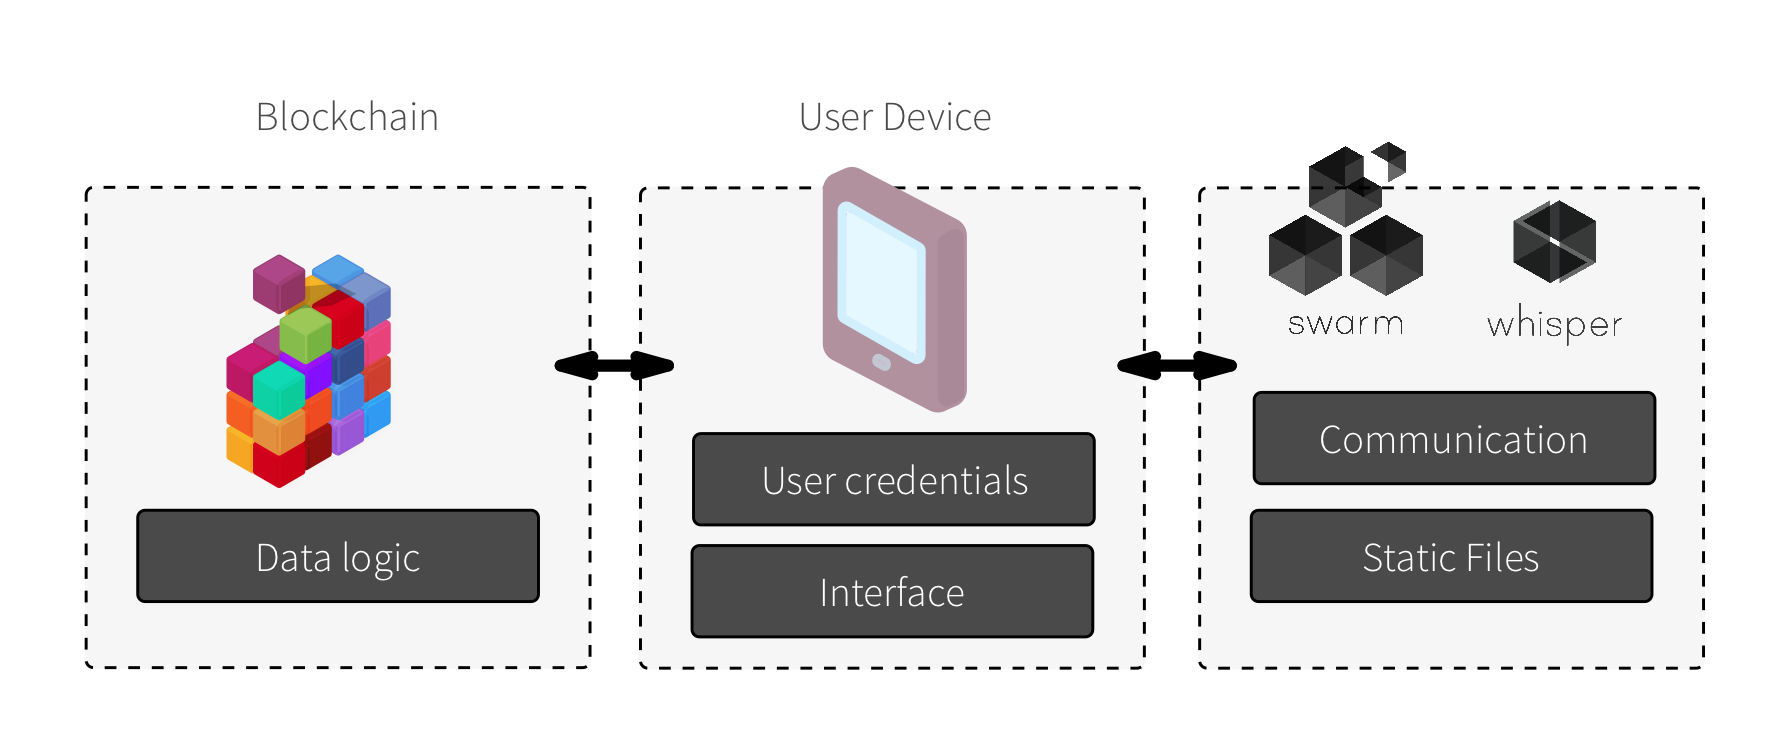
\includegraphics[width=0.75\textwidth]{ethereum-arch-model.png}
	\end{figure}
	
	\subsection{Strumenti per lo sviluppo}
	%https://blog.ethereum.org/2016/07/12/build-server-less-applications-mist/
	Ethereum vuole superare l'approccio client-server che contraddistingue gran parte delle applicazioni di rete, nelle quali troviamo un server, in cui risiedono la logica applicativa, i file statici, le credenziali dell'utente, che comunica e scambia dati con il client. Il client diviene quindi solo un interfaccia per usufruire dei servizi del server. 
	
	Un'architettura più decentralizzata, come quella di Ethereum, ci permette di disporre di un insieme di macchine e di protocolli che permettono di dividere compiti e componenti del sistema, ridistribuendone alcuni sulla macchina del client e altri in una rete peer-to-peer. Come si può osservare dalla figura \ref{fig:ethereum-arc-model}, il layer data, il quale si occupa della gestione dei dati, è affidato in mano agli smart-contract sulla blockchain, i file statici sono forniti tramite \textit{Swarm} e la comunicazione in tempo reale è gestita dal protocollo \textit{Whisper}\footnote{Whisper: è una parte del protocollo peer-to-peer di Ethereum che permette di far comunicare gli utenti attraverso lo stesso mezzo usato dalla blockchain \url{https://github.com/ethereum/wiki/wiki/Whisper}}. Il client interagirà con l'interfaccia per l'applicazione, ma dovrà gestire l'autenticazione. 
	Distribuendo l'autenticazione all'utente e affidandosi alla crittografia si solleva un server centrale della responsabilità di gestire la sicurezza di tutti i client. La distribuzione dei contenuti e la fruizione di protocolli peer-to-peer permettono di ridurre i costi e migliorare l'efficienza dei servizi.
	La divisione del layer di data con quello di presentazione permette di dare la possibilità a chiunque di personalizzare e diffondere una propria interfaccia per la stessa applicazione.

	Di seguito vengono riportati alcune componenti del sistema di Ethereum.\\
		
	\textbf{Mist}\\
	
	Mist viene presentato come l'interfaccia grafica o GUI di Ethereum o il browser per navigare nel Web 3.0 delle Dapp. In pratica è un cointaner Electron connesso a una piattaforma Meteor che permette quindi la totale programmazione degli applicativi come pagine web ( javascript,html e css ). Con esso è possibile interagire con Swarm e reperire le interfacce grafiche per le applicazioni distribuite. \\
	
	\textbf{Electrum-wallet}\\
	
	Il wallet in generale è un'applicazione che consente di connettersi ad una rete blockchain ed effettuare svariate operazioni tra cui inviare, verificare pagamenti e interagire con la blockchain tramite RPC.
	Nel caso specifico di Ethereum-wallet esso è un wallet ma è implementato come Dapp e non come applicazione stand-alone. Essendo una Dapp è stata creata per essere eseguita con meteor, è ottenibile tramite repo \footnote{\url{https://github.com/ethereum/meteor-dapp-wallet}} o via Swarm mediante Mist.\\
	
	\textbf{Swarm}\\
	
	Swarm è un piattaforma distribuita di storage oltre che un servizio di distribuzione dei contenuti, è implementato nativamente nello stack applicativo del web3 di Ethereum. Il principale obiettivo di Swarm è di provvedere una piattaforma di salvataggio distribuita e ridontante per i file relativi alle interfacce delle Dapp, che permetta l'upload di contenuti senza richiedere che il nodo debba restare connesso alla rete di peer.
	Dal punto di vista dell'utente, Swarm non è diverso dal WWW, eccetto che l'invio di informazioni non è verso uno specifico server, ma al sistema di peer. Dal punto di vista oggettivo è una piattaforma di storage peer-to-peer e fornisce soluzioni che sono resistenti a DDOS, censura, downtime e sono tolleranti ai guasti e implementano un sistema di incentivazione e di scambio della criptovaluta comune a tutte le blockchain. Swarm implementa il protocollo di rete di Ethereum devp2p e il sistema DNS di Ethereum.\\
		

\subsection{Problemi delle applicazioni basate su blockchain}\label{ssec:prolemibasatisublockchain}

La blockchain, come già riportato, è un database immutabile e non consente la modifica di un dato registrato a meno di non implementare determinati meccanismi. Questo problema trasportato in Ethereum e nel paradigma dei contratti porta all'immutabilità del codice dei contratti che sono caricati sulla blockchain. Il seguente problema verrà risolto nel sotto capitolo \ref{sssec:systemofcontracts}. Un' altra problematica di ogni applicazione di Ethereum è l'assenza della possibilità di implementare un oracolo, un generatore di numeri casuali, nella EVM di Ethereum. 
%troppo random
Il problema in prima istanza è il fallimento del consenso, della rete di nodi, sull'accettare un blocco che contiene un contratto che ha generato ed effettuato un'operazione su un valore ipoteticamente random. La funzione pseudocasuale porterà ogni nodo a determinare un valore diverso portando al rifiuto del blocco.
%poco random
Viceversa se l'oracolo è deterministico non è possibile implementare tutti quei servizi che si basano sull'estrazione casuale di un numero. 

Sulla rete si trova una soluzione \footnote{\url{https://gist.github.com/alexvandesande/259b4ffb581493ec0a1c}}a questo problema che contempla una particolare implementazione di uno smart contract e l'uso di una funzione deterministica per la generazione del numero pseudocausale. La soluzione viene trattata considerando un problema reale: la vendita di biglietti(ticket) per una lotteria a premi. Definiamo con $t[i]$ il numero del ticket comprato, con $n$ l'altezza del blocco dopo la quale l'estrazione può essere attuata e $x$ il numero di blocchi precedenti ad $n$ su cui è calcolato il numero pseudorandom(eseguento l'hash e l'operazione di modulo sui risultati ottenuti). La vendita di ticket avviene fino al blocco $t\equiv n - x - 1$ dopo il quale lo smart contract nega la vendita. Ogni utente disporrà quindi di ticket su cui non potrà inferire prima dell'estrazione finale, in quanto il calcolo sarà basato sulla creazione dei blocchi successivi a $t$. I miner potranno influenzare l'estrazione attraverso la creazione di nuovi blocchi ma non potranno decidere quale preciso ticket verrà estratto.\\

%contract alarmclock e oraclize
La EVM non ha accesso alla rete e a funzioni dipendenti dal sistema operativo che la ospita in quanto è isolata. Questo oltre a mantenere al sicuro l'esecuzione degli smart contract rappresenta, però, un problema di tutte le blockchain. Basti pensare a un contratto che vuole stimare il costo reale di un servizio, l'Ether ha un tasso di cambio e varia in funzione dell'andamento del Forex delle criptovalute. 
Oltre a questo possiamo essere interessati a richiamare la funzione di un contratto a fronte di un certo evento che può essere il superamento di una certa data temporale. 

Per questo ultimo scopo risiede nella rete principale un contratto, \textit{Ethereum Alarm-clock}\footnote{\url{http://www.ethereum-alarm-clock.com/}} che consente di schedulare eventi tra contratti e di permettere la verificabilità delle invocazioni. L'implementazione presenta alcune caratteristiche e funzionalità che consentono di prevenire l'abuso di questo contratto, ma ovviamente esso si affida all'esecuzione di processi esterni\footnote{Come recita la documentazione: `` Execution guarantees: You may have noted at this point that this service relies on external parties to initiate the execution of these transactions. This means that it is possible that your transaction will not be executed at all. In an ideal situation, there is a sufficient volume of scheduled transactions that operating a server to execute these transactions is a profitable endeavor. The reality is that I operate between 3-5 execution servers dedicated filling this role until there is sufficient volume that I am confident I can turn those servers off or until it is no longer feasible for me to continue paying their costs''.}.


Un altro sistema esterno alla blockchain che permette di disporre maggiori funzionalità, rispetto al sistema Alarm-clock, è \textit{Oraclize}\footnote{\url{http://www.oraclize.it/}}, esso si presenta come il gateway verso Internet per le blockchain per Ethereum e Bitcoin. E' un sistema molto complesso che permette di predisporre di un contratto e di API con le quali si accede alle funzionalità infinite della rete\footnote{ Utili api che possono essere utilizzate attraverso Oraclize sono per esempio quelle di Wolframaplha  \url{https://docs.oraclize.it/\#ethereum-integration-simple-query}}. In Internet l'autenticità e l'integrità dei dati via web viene garantità dall'utilizzo del protocollo https e terze parti fidate (CA come Verisign, GlobalSign, ecc.). Questa architettura si contrappone all'infrastruttura trust-less che risiede nelle blockchain ed Oraclize punta a sostituire l'autenticità dei dati, effettuata mediante terze-parti, con l'\textit{authenticity proof}.


	\subsection{Sviluppare in Solidity}\label{sssec:sviluppareinsolidity}
	% https://blog.aragon.one/library-driven-development-in-solidity-2bebcaf88736#.aleyub1u2
	%https://solidity.readthedocs.io/en/develop
	Abbiamo visto che la EVM esegue un proprio bytecode, infatti è possibile programmare in assembly-ethereum il proprio contratto. Ovviamente ciò è complicato e richiederebbe fin troppo tempo a scrivere un programma efficiente e la manutenibilità sarebbe difficile da ottenere.
	Per questo sono stati creati linguaggi di più alto livello, come Serpent, Viper e Solidity, che permettono la stesura di codice ad alto livello che una volta compilato può essere eseguito nella rete Ethereum.
	
	In generale la EVM ha delle limitazioni:
		\begin{enumerate}
			\item è isolata dal sistema operativo e un altra funzione di un altro contratto e invocabile solo se si conosce il suo indirizzo e la relativa interfaccia (ABI).
			\item Ogni istruzione della EVM ha un costo e l'esecuzione può sollevare un'eccezione in base alla quantità di \textit{GasLimit} contenuta nella transazioni, non possono essere eseguite operazioni intensive.
			\item Una volta creato il contratto non è possibile modificarlo. 
		\end{enumerate}
			
	%https://ethereumclassic.github.io/blog/2017-03-13-viper/ unsafe
	La scelta di quale linguaggio utilizzare è ricaduta su Solidity, che è un linguaggio ad alto livello orientato ai contratti staticamente tipizzato, che permette di scrivere smart contract che supportano l'ereditarietà, implementano funzioni di librerie esterne e utilizzano nuovi tipi definiti dall'utente. Solc è il compilatore per il linguaggio Solidity consente, dati una serie di contratti, di produrre il bytecode per la EVM, la documentazione, le interfacce abi. %https://www.npmjs.com/package/solc
	%descrizione di solidity
	
	Prima di discutere delle innovazioni che porta è bene far precedere dei concetti di questo linguaggio.
		
\begin{lstlisting}
contract A{
	uint amount;
	function A() payable {
		B b = new B();
		amount=msg.value - b.bbb();
	}
}

contract B{
	function bbb() returns (uint){
		return 42;
	}
}
\end{lstlisting}
		
		La principale entità che può essere creata è il contratto e, come i linguaggi OOL, esso presenta un costruttore, una funzione omonima che viene richiamata solo durante il deploy del contratto, le altre funzioni potranno essere invocate in ogni altro momento su un'istanza del contratto.
		
		Eseguendo il codice nella rete di Ethereum ovviamente avremo a disposizione una sintassi e dei costrutti specifici per gestire i pagamenti ai contratti: la label $payable$ informa al compilatore che la funzione $a()$ può accettare $b$ Ether da una transazione e l'istruzione $msg.value$ restituirà l'ammontare $b$.
		
		I contratti dispongono della possibilità di interagire tra di loro comunicando tramite le medesime modalità con le quali un account esterno interagisce con un contratto (call esterna) oppure mediante chiamate speciali che consentono di eseguire funzioni nell'ambiente del contratto chiamante (delegate-call)\footnote{Per maggiori informazioni: \url{http://solidity.readthedocs.io/en/develop/introduction-to-smart-contracts.html?highlight=delegatecall\#delegatecall-callcode-and-libraries}}.
		
		La prima modalità è una chiamata nella quale un contratto può specificare la quantità rimanente di gas nel GasLimit per la chiamata, l'ammontare di Ether da inviare e il payload. Il contratto ricevente, che può essere lo stesso chiamante, allocherà nuova memoria e potrà accedere al payload per eseguire la chiamata.
		Viceversa una delegate-call eseguirà le funzioni nell'ambiente del contratto chiamante e quindi l'ammontare del gas rimasto e per esempio le chiamate a libreria come $msg.value, msg.sig$ e tutte le altre proprietà di $msg$ riporteranno lo stesso valore.
		
		L'innovazione progettuale di Solidity si fonda proprio sull'utilizzo di librerie e sull'invocazione di delegate-call verso esse.

		I contratti come tutti gli account di Ethereum vengono referenziati tramite il loro indirizzo univoco a 160 bit e l' \textit{application binary interface} (ABI).
	
		\begin{multicols}{2}
			 Interfaccia:
			\begin{lstlisting}
[{"constant":false
,"inputs":[]
,"name":"addr"
,"outputs":[{"name":""
			  ,"type":"address"}]
,"payable":false
,"type":"function"}]
			\end{lstlisting}
			\columnbreak
			Codice:
			\begin{lstlisting}
contract A{
	function addr() returns (address){
		return msg.sender;
	}
}
			\end{lstlisting}
		\end{multicols}
		
		%https://github.com/ethereum/wiki/wiki/Ethereum-Contract-ABI
		L'ABI di un contratto è statica e viene determinata in fase di compilazione; è composta dai nomi delle chiamate a funzione, dai tipi degli argomenti e dai valori di ritorno, nonchè eventualmente da precondizioni, postcondizioni e invarianti.
		
		Dopo quest'introduzione su alcune funzionalità del linguaggio possiamo trattare le librerie e il $library driven developement$ in Solidity.
		
		Una libreria è un contratto che non può avere un bilancio in Ether, questo viene assicurato dal compilatore e tutte le chiamate a funzione verso esso sono delle delegate-call.
				 %  using CounterLib for CounterLib.Counter;
				 % self
		Il deploy di un contratto consiste nell'effettuare una transazione speciale con il bytecode del contratto inserito nel payload verso un indirizzo speciale.
		Il bytecode ottenuto dalla compilazione di un contratto, che dipende da una libreria pre-caricata nella blockchain, non può essere registrato su di essa perché l'indirizzo della libreria deve essere linkata nel bytecode del contratto. 
		
		Nel caso di un contratto che utilizza una libreria chiamata Library potremmo trovare nel bytecode un place holder simile a \_\_Untitled:Library\_\_\_\_ che indica il punto in cui inserire l'indirizzo della libreria contenuta nella blockchain.
	 
		Il paradigma della blockchain applicato al codice è di dare la possibilità di usufruire di qualsiasi libreria scritta e registrata da altri, risparmiando il costo e lo spazio sulla catena con la conseguenza di poter disporre di librerie sicure.
		
		Inoltre il paradigma dove ogni operazione ha un costo può essere utilizzato per disincentivare gli account (esterni e non) a non abusare della rete. In Solidity la funzione \lstinline|return;| trova il suo utilizzo nelle call, nelle chiamate che non hanno side-effect\ref{appendice:c}. Il comando interrompe l'esecuzione di una funzione e la EVM ritorna all'esecuzione del codice chiamante, se esistente, se no ritorna il valore alla console. La funzione \lstinline|throw;| invece solleva un eccezione: nel caso di call(dove non viene eseguita una transazione) non viene consumato del gas/ether, ma nel caso di transazioni consuma tutto il gas inserito nella transazione(normalmente se avanza del gas da una computazione viene restituito il rimanente). Il comando \lstinline|throw;| può essere catturato mediante catch, ma se viene propagato può essere usato come strumento per punire economicamente un account.
		
		Solidity è un linguaggio creato recentemente, esso è in fase di sviluppo e tante operazioni non sono possibili, per esempio non è possibile restituire un'istanza di un tipo creato da una funzione e non esistono i tipi primitivi double e float.
		A prescindere da ciò Solidity e la blockchain introducono un interessante modo di sviluppo di applicazioni distribuite. 
		
